% https://tex.stackexchange.com/a/247918
\documentclass{beamer}
\usetheme{Warsaw}
\usecolortheme{orchid}

\usepackage{tikz}
\usetikzlibrary{shadows}
\usetikzlibrary{shapes.arrows}

\begin{document}

    \begin{frame}[plain]
        \frametitle{Conjectures on correspondence and lifting}

        \begin{block}{Theorem 3 (obtained in 1)}
            A relation of dimensions between S and S
        \end{block}

        \begin{columns}
            \begin{column}{.1\textwidth}
            
\begin{tikzpicture}[>=stealth, rotate border/.style={shape border uses incircle, shape border rotate=270}]
                    \node[rotate border=-40, fill=black, minimum height=1.5cm, single arrow, single arrow head extend=.3cm, single arrow head indent=.1cm, inner sep=1.5pt] (arrow) {};
                \end{tikzpicture}
            \end{column}
            \begin{column}{.8\textwidth}
                \begin{alertblock}{}
                    \begin{itemize}
                        \item Definition
                        \item Conjection
                    \end{itemize}
                \end{alertblock}
            \end{column}
        \end{columns}

        \begin{block}{Theorem 3' (new version of Theorem 3)}
            dim S
        \end{block}

        \begin{columns}
            \begin{column}{.1\textwidth}
            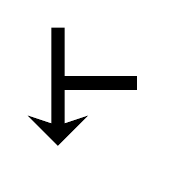
\begin{tikzpicture}[>=stealth, rotate border/.style={shape border uses incircle, shape border rotate=270}]
            \node[rotate border=-40, fill=black, minimum height=1.5cm, single arrow, single arrow head extend=.3cm, single arrow head indent=.1cm, inner sep=1.5pt] (arrow) {};
          \draw[line width=5pt] (0,0) -- (1,0);
            \end{tikzpicture}
            \end{column}
            \begin{column}{.8\textwidth}
                (The RHS suggest ...)
            \end{column}
        \end{columns}       

        \begin{alertblock}{Conjectures}
            ""Correspondance and Lifting""
        \end{alertblock}

    \end{frame}

\end{document}
